\documentclass{article}

%\usepackage{times}
\usepackage{amsmath,amssymb}
\usepackage{amsthm}      % for theorem environment
\usepackage{hyperref}    % for clickable refs
\usepackage{mathtools}   % for dcases
\usepackage{enumerate}


\usepackage[authoryear,sort]{natbib}
\usepackage[usenames,dvipsnames]{color} % For named colors.
\hypersetup{
    unicode=false,          % non-Latin characters in Acrobat’s bookmarks
    pdftoolbar=true,        % show Acrobat’s toolbar?
    pdfmenubar=true,        % show Acrobat’s menu?
    pdffitwindow=false,     % window fit to page when opened
    pdfstartview={FitH},    % fits the width of the page to the window
    pdfnewwindow=true,      % links in new window
    colorlinks=true,        % false: boxed links; true: colored links
    linkcolor=red,          % color of internal links (change box color with linkbordercolor)
    citecolor=BrickRed,     % color of links to bibliography
    filecolor=BurntOrange,  % color of file links
    urlcolor=blue           % color of external links
}

\usepackage[margin=2.5cm]{geometry}

\usepackage{graphicx}
\graphicspath{{./gfx/}}
\DeclareGraphicsExtensions{.eps}
\usepackage{epstopdf}

%\usepackage[nott]{inconsolata} % for C++ code

% C++ styles.
%\newcommand{\cppfont}{\fontfamily{fi4}\selectfont}
%\newcommand{\cppkey}[1]{{\color{blue}#1}}
%\newcommand{\cppclass}[1]{{\color{mint}#1}}
%\newcommand{\cppparam}[1]{{\color{gray}#1}}

% Math
\newcommand{\slfrac}[2]{\left. #1 \middle/ #2 \right.}

% ~~ Theorems and such ~~
\newtheorem{theorem}{Theorem}
\newtheorem{lemma}{Lemma}
\newtheorem{corollary}{Corollary}
\newtheorem{proposition}{Proposition}
\theoremstyle{definition} %% or \theoremstyle{remark} will produce roman text
\newtheorem{definition}{Definition}
\newtheorem{remark}{Remark}

% ~~ Math operators ~~
\DeclareMathOperator{\EV}{\mathbf{E}} % expected value
\DeclareMathOperator{\Var}{\mathbf{Var}} % variance
\DeclareMathOperator{\Cov}{\mathbf{Cov}} % covariance
\DeclareMathOperator{\Corr}{\mathbf{Corr}} % correlation
\DeclareMathOperator{\SD}{\mathbf{s.d.}} % standard deviation

% ~~ Distributions ~~
\DeclareMathOperator{\DNorm}{\mathcal{N}} % normal distribution
\DeclareMathOperator{\DLogNorm}{\ln \DNorm } % normal distribution
\DeclareMathOperator{\DExp}{\mathrm{Exp}} % exponential distribution
\DeclareMathOperator{\DPareto}{\mathrm{Pareto}} % exponential distribution
\DeclareMathOperator{\DBeta}{\mathrm{Be}} % exponential distribution
\DeclareMathOperator{\DUnif}{\mathrm{Uniform}} % exponential distribution
\newcommand{\scbeta}[1]{\DBeta_{\left(0, #1\right)}} % scaled beta distribution

% ~~ Misc ~~
\newcommand{\ignore}[1]{}
\newcommand{\nolabel}[1]{}
\newcommand{\Mode}{\theta}

\begin{document}

\section{Overview}

    A trivial extension of the ziggurat algorithm which is suitable for continuous symmetric unimodal distributions will be presented. This is a summary of \citet{Marsaglia+Tsang} and \citet{Doornik:05}.
    Let $\Mode $ denote the mode of the distribution, and $T(x)$ denote the tail function:
    \[
        T(x) = \int _x ^{\infty} f(t) \,dt.
    \]
    Note that normalizing the density function (so that $T(-\infty ) = 1$) is not necessary.

\subsection{Monotone decreasing density}

    First consider the interval to the right of the mode, where the density function, $f$, is decreasing.
    The goal is to cover the density function by $n \ge 2$ boxes of the same volume and the following form:
    \begin{align*}
        B_0 &= \{ (x, y) \,:\, x \ge \Mode , \, 0 \le y \le \min (f(x_1), f(x)) \}, \\
        B_k &= [\Mode , x_k] \times [f(x_k), f(x_{k + 1})], \quad 1 \le k \le n - 2, \\
        B_{n - 1} &= [\Mode , x_k] \times [f(x_k), f(\Mode )].
    \end{align*}
    Note that the bottom box is the only non-rectangular.
    %
    \begin{figure*}[!htb]
        \centering
        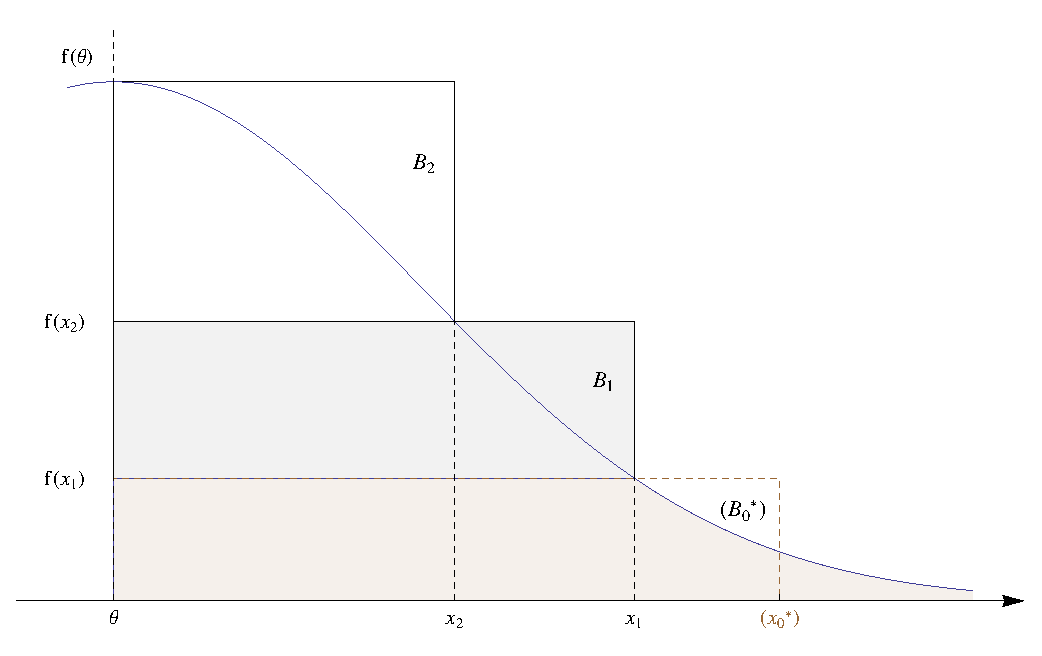
\includegraphics[width=0.6\textwidth]{ziggurat_normal_3.eps}
        \caption{Illustration of one-sided ziggurat algorithm when $n = 3$.}
        \label{fig:ziggurat_normal_3}
    \end{figure*}

    Since the area of each box is to be the same as the area of $B_0$, one gets a (non-linear) system of $n$ equations
    \begin{align} \label{eq:zigg_system}
        \begin{dcases}
            V &= (x_1 - \Mode ) f(x_1) + T(x_1) \\
            V &= (x_1 - \Mode ) \left(f(x_2) - f(x_1)\right) \\
            V &= \quad \cdots \\
            V &= (x_{n - 2} - \Mode ) \left(f(x_{n - 1}) - f(x_{n - 2})\right) \\
            V &= (x_{n - 1} - \Mode ) \left(f(\Mode ) - f(x_{n - 1})\right)
        \end{dcases}
    \end{align}
    with $n$ unknowns. Put otherwise, $V = (x_1 - \Mode ) f(x_1) + T(x_1) = (x_{n - 1} - \Mode ) \left(f(\Mode ) - f(x_{n - 1})\right)$, and
    \begin{align*}
        x_{k + 1} &= f^{-1} \left( f(x_k) + \frac{V}{x_k - \Mode } \right) \quad \text{for $1 \le k \le n - 2$}.
    \end{align*}

    \begin{proposition}
        Due to the assumption of monotonicity, system \eqref{eq:zigg_system} has a unique solution.
    \end{proposition}

    \ignore{
    As it is a covering, $V \ge T(\Mode ) / n$ and one can get an upper bound $\overline{x}_1$ for $x_1$:
    \begin{align}
        (\overline{x}_1 - \Mode ) f(\overline{x}_1) + T(\overline{x}_1) = T(\Mode ) / n.
    \end{align}
    %
    If a lower bound is necessary, one could solve the system \eqref{eq:zigg_system} for $n = 2$:
    \begin{align}
        2 (\underline{x}_1 - \Mode ) f(\underline{x}_1) + T(\underline{x}_1) = (\underline{x}_1 - \Mode ) f(\Mode ).
    \end{align}
    } % End of ignore.

\subsection{Symmetric unimodal density}

    When the density is unimodal and symmetric about its mode $\Mode $, first solve \eqref{eq:zigg_system} for the right tail to get $\{ B_{n - 1}, \cdots , B_0 \}$ and the corresponding partition $\{ \Mode , x_{n - 1}, \dots, x_1  \}$.
    One option would be to sample from the right tail, and then use an unused bit from one of the generated random numbers to determine whether to replace the generated variable $z$ with $\Mode - z$.
    
    Alternatively, if doubling the size of lookup tables is not an issue, one could reflect the boxes about $\Mode $ to get the resulting partition for $2 n$ boxes $\{ B_{2n - 1}, \cdots , B_n, B_{n - 1}, \cdots , B_0 \}$:
    \[
        \{ 2 \Mode - x_1, 2 \Mode - x_2, \dots, 2 \Mode - x_{n - 1}, \Mode , x_{n - 1}, \dots, x_2, x_1 \};
    \]
    write $x_{n + i} = 2 \Mode - x_{n - 1 - i}$ for $0 \le i \le n - 2$ so that each $B_j$ (apart from the tail boxes) has $x_j$ for either left or right abscissa. We will adopt this extended lookup table approach.

\section{The ziggurat algorithm}

    The algorithm of \citet{Marsaglia+Tsang} and \citet{Doornik:05} is summarized below (trivially extended to the symmetric case with $2 n$ boxes).\ignore{We propose using extended lookup tables, which would allow to avoid scaling of random numbers and calculating absolute values, thus improving both accuracy and performance.}

    First, introduce an auxiliary \emph{rectangular} box $\left( B_0^* \right)$ corresponding to $B_0$, so that it has the same height and volume, and denote
    \[
        x_0 \triangleq \Mode + V / f(x_1), \qquad x_{2 n - 1} \triangleq \Mode - V / f(x_1) = 2 \Mode - x_0.
    \]

\subsection{Continuous generators}
    Pre-compute the following properties for the $2 n$ boxes:
    \begin{enumerate}[(i)]
        \item Box width $w$ (signed: positive for right tail and negative for left), height $h$, and bottom ordinate $b$:
            \begin{align*}
                w_i = x_i - \Mode , \quad h_i = \big| f(x_i) - f(x_{i + 1}) \big|, \quad b_i = f(x_i)
            \end{align*}
            for $0 \le i \le 2 n - 1$. In the case of tail boxes, $w$, $h$ and $b$ lose their intuitive meaning; but the former is mathematically convenient, whereas the latter two are plainly not used.

        \item Probabilities $q$ of ``simple coverage'':
            \begin{align*}
                q_i &= \slfrac{w_{i + 1}}{w_{i}} \quad \text{for} \quad 0 \le i \le n - 1, \\
                q_i &= \slfrac{w_{i}}{w_{i + 1}} \quad \text{for} \quad n \le i \le 2 n - 1.
            \end{align*}
    \end{enumerate}

    We are now ready to present the main algorithm.
    \begin{enumerate}
        \item \label{item:alg:choose_box} Generate the zero-based box index $I \sim \DUnif (\{ 0, 1, \cdots , 2 n - 1 \})$.

        \item \nolabel{item:alg:horizontal} Generate $U \sim \DUnif ([0, 1))$, and let $z = \Mode + U \cdot w_I$.

        \item \nolabel{item:alg:inside_simple} If $U < q_I$ accept $z$.

        \item %
            \begin{enumerate}
                \item \label{item:alg:tail_box} If $I = 0$, accept a $v$ from the right tail (in the normal case see, e.g., \citet{Marsaglia:64}); for the left tail, i.e., when $I = 2 n - 1$, accept $2 \Mode - v$.

                \item If $1 \le I \le 2 n - 2$, generate $V \sim \DUnif ([0, 1))$, and if $b_I + V \cdot h_I < f(z)$ accept $z$.
            \end{enumerate}

        \item Otherwise return to step \ref{item:alg:choose_box}.
    \end{enumerate}
    This is a sample-rejection type algorithm; note that step \ref{item:alg:tail_box} is essential because $\left( B_0^* \right)$ does \emph{not} cover the tail.
    Note also, that $w_j = -w_{2n - 1 - j}$ and $(\cdot ) _j = (\cdot ) _{2n - 1 - j}$ for $(\cdot ) \in \{ h, b, q \}$, $0 \leq j \leq n - 1$.

\subsection{Discrete generators}
    In practice one usually has to deal with $m$-bit integer generators.
    The main algorithm can be adjusted to take advantage of integer arithmetic in the following way:
    \begin{enumerate}
        \item \label{item:alg:choose_box_discr} Generate the zero-based box index $I \sim \DUnif (\{ 0, 1, \cdots , 2 n - 1 \})$.

        \item \nolabel{item:alg:horizontal} Generate $U \sim \DUnif (\{ 0, \cdots , 2^m - 1 \})$, and let $z = \Mode + U \cdot (2^{-m}\, w_I)$.

        \item \nolabel{item:alg:inside_simple} If $U < \lfloor 2^m \, q_I \rfloor$ accept $z$.

        \item %
            \begin{enumerate}
                \item \nolabel{item:alg:tail_box} If $I = 0$, accept a $v$ from the right tail (in the normal case see, e.g., \citet{Marsaglia:64}); for the left tail, i.e., when $I = 2 n - 1$, accept $2 \Mode - v$.

                \item If $1 \le I \le 2 n - 2$, generate $V \sim \DUnif (\{ 0, \cdots , 2^m - 1 \})$, and if $b_I + V \cdot (2^{-m}\, h_I) < f(z)$ accept $z$.
            \end{enumerate}

        \item Otherwise return to step \ref{item:alg:choose_box_discr}.
    \end{enumerate}
    Thus, instead of storing $w$ and $h$ we can store $2^{-m}\, w$ and $2^{-m}\, h$, and instead of $q$---integer-valued $\lfloor 2^m \, q \rfloor$; $b$ stays intact. To summarize, we store:
    \begin{enumerate}[(i)]
        \item Down-scaled box width $\tilde{w}$, down-scaled height $\tilde{h}$, and bottom ordinate $b$:
            \begin{align*}
                \tilde{w}_i = 2^{-m}\, (x_i - \Mode ), \quad \tilde{h}_i = 2^{-m}\, \big| f(x_i) - f(x_{i + 1}) \big|, \quad b_i = f(x_i)
            \end{align*}
            for $0 \le i \le 2 n - 1$.

        \item Up-scaled probabilities $\hat{q}$ of ``simple coverage'':
            \begin{align*}
                \hat{q}_i &= \left\lfloor 2^m \, \slfrac{w_{i + 1}}{w_{i}} \right\rfloor \quad \text{for} \quad 0 \le i \le n - 1, \\
                \hat{q}_i &= \left\lfloor 2^m \, \slfrac{w_{i}}{w_{i + 1}} \right\rfloor \quad \text{for} \quad n \le i \le 2 n - 1.
            \end{align*}
    \end{enumerate}
    Note that $\lceil \log _2 (2 n) \rceil$ bits are used for $I$; thus the remaining $2^{m} - \lceil \log _2 (2 n) \rceil$ bits may be used to enhance $U$---or may they?


\bibliographystyle{plainnat}
\bibliography{ziggurat}


\end{document}
